\subsection*{Экспериментальная установка}

Схема экспериментальной установки изображена на рис. \ref{fig:exp}. На рисунке обозначены:
А -- амперметр;
Б7-4 -- стабилизированный источник питания (подаёт напряжение накала);
$K_1$ -- тумблер для включения в цепь источника Б7-4;
Б5-10 -- выпрямитель (подаёт на анод ускоряющее напряжение);
$Pi_3$ -- потенциометр, регулирующий величину ускоряющего напряжения;
$V_1$ -- вольтметр, измеряющий величину ускоряющего напряжения;
4,5 В -- батарея КБСЛ, -- источник задерживающего потенциала;
$Pi_2$ -- потенциометр, регулирующий величину задерживающего потенциала;
$V_2$ -- вольтметр, измеряющий величину задерживающего потенциала;
$\mu A$ -- микроамперметр -- регистрирует ток в цепи коллектора;
$K_3$ -- ключ, переключающий схему из статического режима в динамический;
Т -- понижающий трансформатор, -- подаёт ускоряющий потенциал при динамическом режиме.
    % \item - нагрузочный резистор.

\begin{figure}[ht]
    \centering
    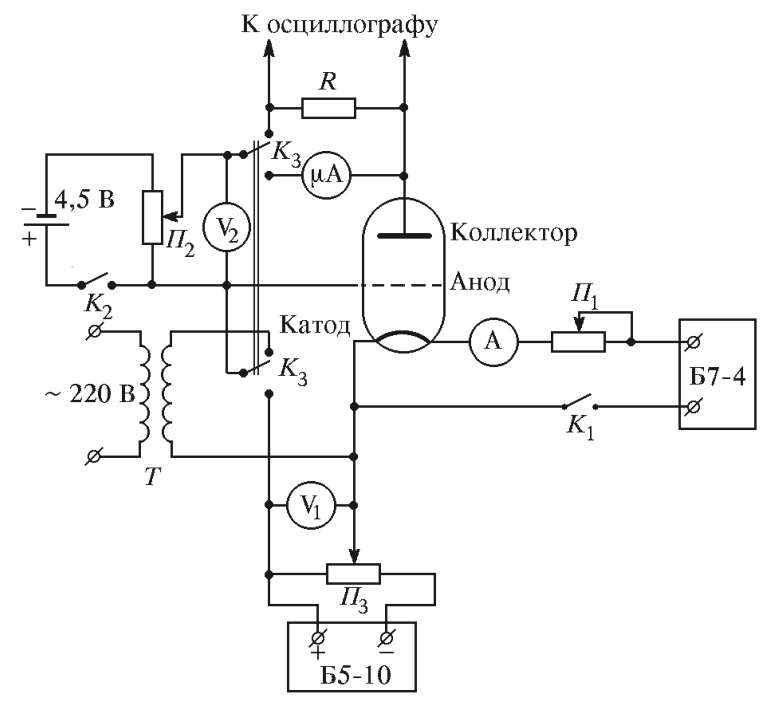
\includegraphics[width=0.5\textwidth]{figures/exp.png}
    \caption{Схема экспериментальной установки}
    \label{fig:exp}
\end{figure}


Разреженный одноатомный газ заполняет трёхэлектродную лампу. Электроны, испускаемые разогретым катодом, ускоряются в постоянном электрическом поле, созданном между катодом и сетчатым анодом лампы. Передвигаясь от катода к аноду, электроны сталкиваются с атомами гелия.